% Options for packages loaded elsewhere
\PassOptionsToPackage{unicode}{hyperref}
\PassOptionsToPackage{hyphens}{url}
%
\documentclass[
]{article}
\usepackage{amsmath,amssymb}
\usepackage{iftex}
\ifPDFTeX
  \usepackage[T1]{fontenc}
  \usepackage[utf8]{inputenc}
  \usepackage{textcomp} % provide euro and other symbols
\else % if luatex or xetex
  \usepackage{unicode-math} % this also loads fontspec
  \defaultfontfeatures{Scale=MatchLowercase}
  \defaultfontfeatures[\rmfamily]{Ligatures=TeX,Scale=1}
\fi
\usepackage{lmodern}
\ifPDFTeX\else
  % xetex/luatex font selection
\fi
% Use upquote if available, for straight quotes in verbatim environments
\IfFileExists{upquote.sty}{\usepackage{upquote}}{}
\IfFileExists{microtype.sty}{% use microtype if available
  \usepackage[]{microtype}
  \UseMicrotypeSet[protrusion]{basicmath} % disable protrusion for tt fonts
}{}
\makeatletter
\@ifundefined{KOMAClassName}{% if non-KOMA class
  \IfFileExists{parskip.sty}{%
    \usepackage{parskip}
  }{% else
    \setlength{\parindent}{0pt}
    \setlength{\parskip}{6pt plus 2pt minus 1pt}}
}{% if KOMA class
  \KOMAoptions{parskip=half}}
\makeatother
\usepackage{xcolor}
\usepackage[margin=1in]{geometry}
\usepackage{longtable,booktabs,array}
\usepackage{calc} % for calculating minipage widths
% Correct order of tables after \paragraph or \subparagraph
\usepackage{etoolbox}
\makeatletter
\patchcmd\longtable{\par}{\if@noskipsec\mbox{}\fi\par}{}{}
\makeatother
% Allow footnotes in longtable head/foot
\IfFileExists{footnotehyper.sty}{\usepackage{footnotehyper}}{\usepackage{footnote}}
\makesavenoteenv{longtable}
\usepackage{graphicx}
\makeatletter
\def\maxwidth{\ifdim\Gin@nat@width>\linewidth\linewidth\else\Gin@nat@width\fi}
\def\maxheight{\ifdim\Gin@nat@height>\textheight\textheight\else\Gin@nat@height\fi}
\makeatother
% Scale images if necessary, so that they will not overflow the page
% margins by default, and it is still possible to overwrite the defaults
% using explicit options in \includegraphics[width, height, ...]{}
\setkeys{Gin}{width=\maxwidth,height=\maxheight,keepaspectratio}
% Set default figure placement to htbp
\makeatletter
\def\fps@figure{htbp}
\makeatother
\setlength{\emergencystretch}{3em} % prevent overfull lines
\providecommand{\tightlist}{%
  \setlength{\itemsep}{0pt}\setlength{\parskip}{0pt}}
\setcounter{secnumdepth}{-\maxdimen} % remove section numbering
\ifLuaTeX
  \usepackage{selnolig}  % disable illegal ligatures
\fi
\usepackage{bookmark}
\IfFileExists{xurl.sty}{\usepackage{xurl}}{} % add URL line breaks if available
\urlstyle{same}
\hypersetup{
  hidelinks,
  pdfcreator={LaTeX via pandoc}}

\author{}
\date{\vspace{-2.5em}}

\begin{document}

\section{I Introduction}\label{i-introduction}

Question: How does the annual salary (USD) vary between different
professions (Data Scientist, Software Engineer, Bioinformatics Engineer)
across different regions (San Francisco and Seattle)?

Interest: Understanding the salary distribution across professions and
regions can provide insightful economic. Insights into wage can help
individuals make informed decisions about career paths and relocation
opportunities. Additionally, businesses and governments can use this
information to strategize their hiring plans and economic policies
respectively.

Approach: Two Factor ANOVA (TFA)

\newpage

\section{III Diagnostics}\label{iii-diagnostics}

In this section, we will check whether our data satisfies the ANOVA
assumptions.

The assumptions are: 1. All samples are independent 2. All groups in
factor \(A\) are independent 3. All groups in factor \(B\) are
independent 4. Errors are normally distributed and have constant
variance where \(ϵ_{ij} \sim N(0, \sigma_\epsilon^2)\)

Due to limitations, we can only test whether the errors are normally
distributed and have constant variance. We cannot determine whether
assumptions one through three are satisfied as we did not sample the
data. For simplicity, we will assume these hold.

\subsection{III.1 Assessing Type I and Type II
Errors}\label{iii.1-assessing-type-i-and-type-ii-errors}

To determine which \(\alpha\) to use for diagnostics, we need to assess
whether we want to minimize the chance of a Type I Error or a Type II
Error.

\begin{itemize}
\tightlist
\item
  Type I Error: When you reject \(H_0\) when in reality \(H_0\) is true.
  In this case, this represents the chance we conclude the data violates
  our ANOVA assumptions when in reality it satisfies our ANOVA
  assumptions.
\item
  Type II Error: When you accept \(H_0\) when in reality \(H_0\) is
  false. In this case, this represents the chance we conclude the data
  satisfies our ANOVA assumptions when in reality it violates our ANOVA
  assumptions
\end{itemize}

For determining normality and constant variance, we want to minimize our
probability of incorrect assumptions, so a Type II error is worse than a
Type I error. As a result, we want to maximize \(\alpha\), so we will
use \(\alpha = 0.1\) as our threshold.

\subsection{III.2 Determine Normality}\label{iii.2-determine-normality}

\subsubsection{III.2.1 QQ Plot}\label{iii.2.1-qq-plot}

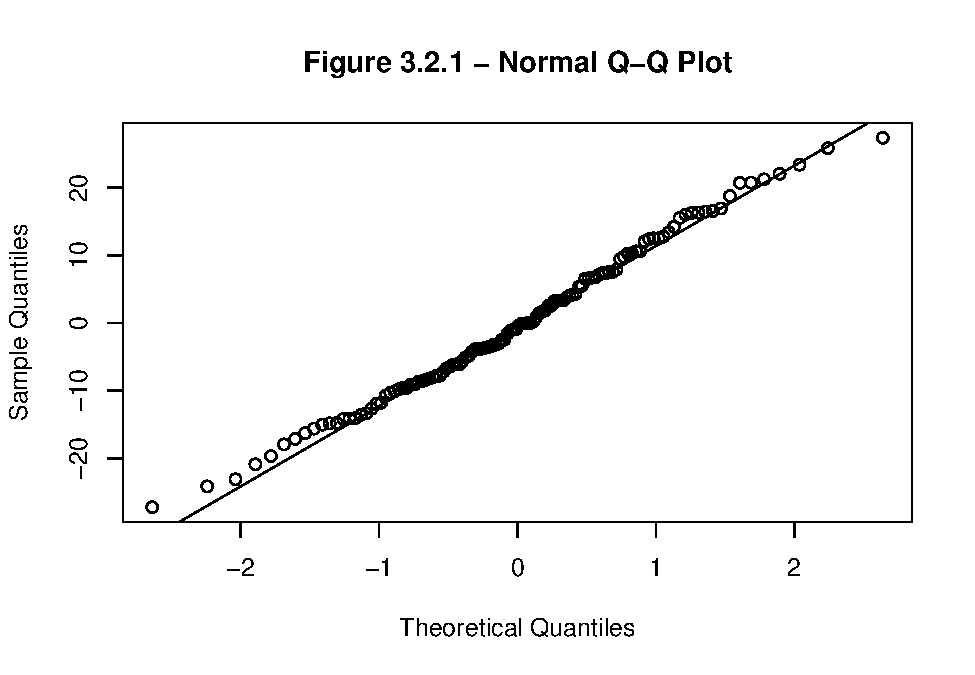
\includegraphics{STA_106_Project_2_files/figure-latex/unnamed-chunk-4-1.pdf}

The QQ plot shows our original data plotted against a theoretical normal
distribution. From the plot, the majority of the data points converge to
the normal line, suggesting that our data is most likely normal. We
formalize this plot by running a Shapiro-Wilk Test next.

\subsubsection{III.2.2 Shapiro Wilk
Test}\label{iii.2.2-shapiro-wilk-test}

\(H_0:\) Our data is normal.

\(H_a:\) Our data is not normal.

\(p = 0.6698\)

Since \(p > \alpha\), we accept \(H_0\). Therefore, our data is normal.

\subsection{III.3 Assessing Constant
Variance}\label{iii.3-assessing-constant-variance}

\subsubsection{III.3.1 Plot on Errors vs Groups
Means}\label{iii.3.1-plot-on-errors-vs-groups-means}

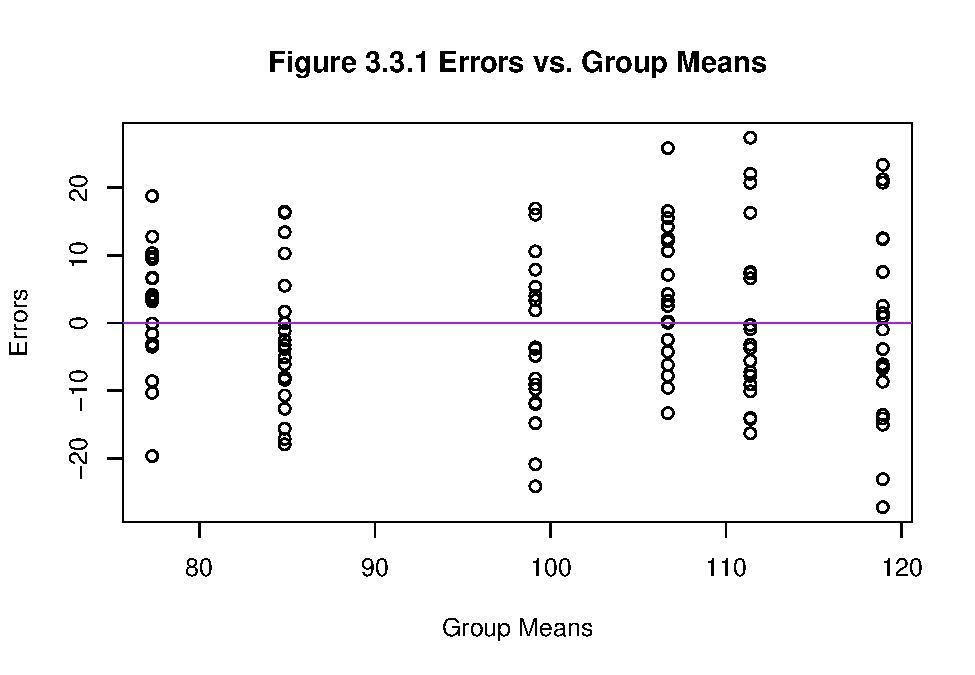
\includegraphics{STA_106_Project_2_files/figure-latex/unnamed-chunk-6-1.pdf}

From figure 3.3.1, the dots for each group mean seem to have
approximately the same spread, suggesting that there is constant
variance between groups. To formalize this, we will run the BF-test
next.

\subsubsection{III.3.2 BF-Test}\label{iii.3.2-bf-test}

\begin{verbatim}
## Warning in leveneTest.default(y = y, group = group, ...): group coerced to
## factor.
\end{verbatim}

\(H_0:\) The data have constant variances.

\(H_a:\) The data does not have constant variances.

Since \(p = 0.3048 > \alpha\), we accept \(H_0\). Therefore, the data
has constant variances.

\subsection{III.4 Final Verdict}\label{iii.4-final-verdict}

We can conclude that the errors are normally distributed and have
constant variances, satisfying one of our ANOVA assumptions. No
transformation nor outlier removal is needed.

\section{IV Analysis and
Interpretation}\label{iv-analysis-and-interpretation}

\subsection{IV.1 Finding Best Model}\label{iv.1-finding-best-model}

We will first observe the conditional \(R^2\) and differences between
mean values to see what to expect. Then we will use F-statistic test to
find out which model to use. When conducting our test, we will first
test for interaction effect. If there is interaction effect, we use the
model with interaction effect and stop the testing. Otherwise, we will
continue testing for factor A and factor B. We will only use these
factors if there are significant effects.

\subsubsection{\texorpdfstring{IV.1.1 Conditional
\(R^2\)}{IV.1.1 Conditional R\^{}2}}\label{iv.1.1-conditional-r2}

\textbf{Figure 4.1.1}

\begin{verbatim}
##           AB    (A+B)        A        B Empty/Null
## SSE 15252.93 16058.34 17764.09 39872.94   41578.69
\end{verbatim}

\textbf{Figure 4.1.2}

\begin{longtable}[]{@{}
  >{\raggedleft\arraybackslash}p{(\columnwidth - 8\tabcolsep) * \real{0.2079}}
  >{\raggedleft\arraybackslash}p{(\columnwidth - 8\tabcolsep) * \real{0.1980}}
  >{\raggedleft\arraybackslash}p{(\columnwidth - 8\tabcolsep) * \real{0.1980}}
  >{\raggedleft\arraybackslash}p{(\columnwidth - 8\tabcolsep) * \real{0.1980}}
  >{\raggedleft\arraybackslash}p{(\columnwidth - 8\tabcolsep) * \real{0.1980}}@{}}
\toprule\noalign{}
\begin{minipage}[b]{\linewidth}\raggedleft
\(R^2(AB&#124;(A+B))\)
\end{minipage} & \begin{minipage}[b]{\linewidth}\raggedleft
\(R^2((A+B)&#124;A)\)
\end{minipage} & \begin{minipage}[b]{\linewidth}\raggedleft
\(R^2((A+B)&#124;B)\)
\end{minipage} & \begin{minipage}[b]{\linewidth}\raggedleft
\(R^2(A&#124;Empty)\)
\end{minipage} & \begin{minipage}[b]{\linewidth}\raggedleft
\(R^2(B&#124;Empty)\)
\end{minipage} \\
\midrule\noalign{}
\endhead
\bottomrule\noalign{}
\endlastfoot
0.0502 & 0.096 & 0.5973 & 0.5728 & 0.041 \\
\end{longtable}

From figure 4.1.2, there seems to be a significant factor A effect since
its \(R^2\) value is large when adding it both to the empty model and
the model with factor B. While the conditional \(R^2\) may hint which
factors may be significant, this is not a conclusive test.

\subsubsection{IV.1.2 Assessing Type I and Type II
Errors}\label{iv.1.2-assessing-type-i-and-type-ii-errors}

To determine which \(\alpha\) to use for diagnostics, we need to assess
whether we want to minimize the chance of a Type I Error or a Type II
Error.

Type I Error: The chance we reject \(H_0\) when in reality \(H_0\) is
true. In this case, it is the chance we conclude that there is a
significant effect when in reality there is no significant effect.

Type II Error: The chance that we accept \(H_0\) when in reality \(H_0\)
is false. In this case, it is the chance we conclude that there is no
significant effect when in reality there is a significant effect.

In our analysis, we want to capture the factor and interaction effects
if it exists, and thus want to minimize unexplained error. The lower the
Type II Error, the less chance of falsely concluding no significant
effect, increasing the chance of less unexplained error. Since a type II
error is worse, we want to minimize it, so we will choose a higher
\(\alpha\) value. As a result, we will choose \(\alpha = 0.1\).

\subsubsection{IV.1.3 Testing for Interaction
Effect}\label{iv.1.3-testing-for-interaction-effect}

Our full model is
\(Y_{ijk} = \mu_{ij} + \gamma_i + \delta_j + (\gamma\delta)_{ij} + \epsilon_{ijk}\)

With constraints: - \(\sum \gamma_i = 0\) - \(\sum \delta_j = 0\) -
\(\sum \sum (\gamma_i \delta_j) = 0\)

Our reduced model is
\(Y_{ijk} = \mu_{ij} + \gamma_i + \delta_j + \epsilon_{ijk}\)

With constraints: - \(\sum \gamma_i = 0\) - \(\sum \delta_j = 0\)

Hypothesis: - \(H_0:\) There is no significant interaction effect
(i.e.~all \((\gamma\delta)_{ij} = 0\)). Do not use the full model. -
\(H_a:\) There is significant interaction effect (i.e.~at least one
\((\gamma\delta)_{ij} \neq 0\)). Use the full model.

Test results: - \(F_s = 3.0098\) - \(p = 0.0532\)

Since \(p \leq \alpha\), we reject \(H_0\). Therefore, we will use the
full model.

\subsubsection{IV.1.4 Model Choice}\label{iv.1.4-model-choice}

From our testing, our final model choice is
\(Y_{ijk} = \mu_{ij} + \gamma_i + \delta_j + (\gamma \delta)_{ij} + \epsilon{ijk}\)

With constraints: - \(\sum \gamma_i = 0\) - \(\sum \delta_j = 0\) -
\(\sum \sum (\gamma_i \delta_j) = 0\)

\subsection{IV.2 Comparisons of Different
Factors}\label{iv.2-comparisons-of-different-factors}

First, we will create pairwise confidence intervals to test how much
professions affects average annual salary. Then, we will create another
pairwise interval to test how much region affects average annual salary.
Lastly, we will create non-pairwise intervals to test for more complex
differences.

\subsubsection{IV.2.1 Accuracy}\label{iv.2.1-accuracy}

We want to minimize the error of our confidence interval for stronger
interpretation. As a result, we want to minimize the probability that
the value does not lie within our confidence interval by minimizing
\(\alpha\). Therefore, we will choose \(\alpha = 0.001\).

\subsubsection{IV.2.2 Multiplier}\label{iv.2.2-multiplier}

We will compute 3 pairwise confidence intervals for group A and 1
pairwise confidence interval for group B to determine the difference in
annual salary given the difference in profession or region. For these
intervals, we can use either the Bonferonni, Tukey, or Scheffe
multipliers. We will pick the smallest multiplier for higher precision.

We will also compute 2 non-pairwise confidence intervals. For these
intervals, we cannot use Tukey since that is for pairwise comparisons
only. We will pick either Bonferonni or Scheffe, whichever one is
smaller.

\subsubsection{IV.2.3 Effect of Profession on Average Annual
Salary}\label{iv.2.3-effect-of-profession-on-average-annual-salary}

We will analyze the difference in average annual salary between all
professions.

Our 99.9\% confidence interval for the difference of average annual
salary between BE (bioinformatics engineer) and DS (data scientist) is
\([-43.6051, -24.5169]\). This means that we are 99.9\% confident that
on average BE makes around 24.5169 to 43.6051 less annually compared to
DS. Since 0 is not in our confidence interval, we are 99.9\% certain
that there is a difference in average annual salary between BE and DS
(i.e.~BS makes less than DS).

Our 99.9\% confidence interval for the difference of average annual
salary between DS and SE (software engineer) is \([2.6974, 21.7856]\).
This means that we are 99.9\% confident that on average DS makes around
2.6974 and 21.7856 more annually compared to SE. Since 0 is not in our
confidence interval, we are 99.9\% certain that there is a difference in
average annual salary between DS and SE (i.e.~DS makes more than SE).

Our 99.9\% confidence interval for the average difference of annual
salary between BE and SE is \([-31.3635, -12.2753]\). This means that we
are 99.9\% confident that on average BE makes around 12.2753 and 31.3635
less annually compared to SE. Since 0 is not in our confidence interval,
we are 99.9\% certain that there is a difference in average annual
salary between BE and SE (i.e.~BE makes more than SE).

\subsubsection{IV.2.4 Effect of Region on Average Annual
Salary}\label{iv.2.4-effect-of-region-on-average-annual-salary}

We will analyze the difference of average annual salary between S and
SF.

Our 99.9\% confidence interval for the average difference of annual
salary between S and SF is \([-14.6743, -0.4066]\). This means that we
are 99.9\% confident that on average people in S makes around 0.4066 and
14.6743 less annually compared to SF. Since 0 is not in our confidence
interval, we are 99.9\% certain that there is a difference in average
annual salary between people in S and SF (i.e.~S makes less than SF).

\subsubsection{IV.2.5 Addressing Large Salary Difference Between Regions
for
SE}\label{iv.2.5-addressing-large-salary-difference-between-regions-for-se}

From the summary, we see there is an interaction effect where SE gets
much higher pay in SF than S compared to other professions. This means
that regional differences may not apply to professions other than SE. We
will use pairwise confidence interval where we compare the effect of
different regions on average annual salary for average professional
other than SE.

Our 99.9\% confidence interval for the average difference in annual
salary between S and SF is \([-12.6901, 4.7841]\) for the average
professional other than SE. Since 0 is in our confidence interval, we
cannot conclude that there is a difference between regions for the
average professional other than SE. Therefore we believe that the result
from IV.2.4, the difference of average annual salary on region, mainly
applies to SE.

\subsubsection{IV.2.6 Addressing Wage Inequality in
SF}\label{iv.2.6-addressing-wage-inequality-in-sf}

From the summary, we noticed a huge gap between the average annual
salary for the lowest paying profession compared to the other
professions. This gap may be a sign of wage inequality. Lets test how
big this gap is.

Our 99.9\% confidence interval for the difference in average annual
salary between BE and the average profession other than BE is
\([-42.2981, -20.8966]\) for SF. This means that we are 99.9\% confident
that in SF the profession BE pays an average annual salary of around
20.8966 to 42.2981 lower than the average other professions. Since 0 is
not in our confidence interval, we conclude that there is a difference
between BE and the average other professions in SF.

\section{V Conclusion}\label{v-conclusion}

In conclusion, we find that the profession does affect annual salary. We
also found that region only affects salary for SE (software engineers).
Lastly, we found a significant wage gap between the lowest paying job,
BE (bioinfograhics enginering), and other professions in SF. We are
confident in our results as our data does not violate normality or
constant variance ANOVA assumptions, and in our diagnostics and we chose
conservative \(\alpha\) values for each test yielding more accurate
results.

One limitation is the fact that we have very few groups and not enough
data. For example, there are other technology roles like Machine
Learning and hardware engineering. We could have also separated entry
level roles from senior level roles. These ideas can present more
insighful results.

\end{document}
